% 06_results.tex -- Chapter 6 Experiments and results (14 pages). Owner: Results writer (plan section 6, step 2).
% Skeleton from REWRITE_PLAN.md section 2. Writing rules: section 5 of the plan.
% "absorbs" = lines of draft_2026-10_original/main.tex (or the named draft file) whose content moves here.

\chapter{Experiments and Results}
\label{ch:results}

% Writer-owned tables used here (input them where they belong, owned by other writers): T8 depth, T9 neck, T10 fingers
% (Diagnostics writer), T11 student recipe (Method writer). Tables owned by this chapter: T12, T15, T16, T17.
% Figures: F6, F7, F9, F13 exist (figures/img/); F10, F11, F12, F17 wait for the student's files (plan section 3).

\section{Setup recap}
\label{sec:res-setup}
% absorbs - (new)
% needs: one paragraph: sets (AnnyOne holdout V1, 3DPW test v23, Relative Human val), settings V0/V1, noise floor (\NoisePVE\,mm, \NoiseHeadDeg\,deg, about \NoiseRecall{} recall points), one run per arm
\TODO{Sets, settings, noise floor, one run per arm and no seed.}

\section{Depth fix: pilots and final model}
\label{sec:res-depth}
% absorbs - (new; draft has nothing on the depth bug)
% needs: T8 (Diagnostics writer), F7, F8 (appendix), F15; root 1.21 -> 0.54 m (pilot), 1402 -> 728 mm (Final vs Control); slope 0.42; size 0.78; pelvis px 26.7 -> 41.1 (H 3.1). Rule: quote the absolute root error, never the signed offset; "the fix moved the offset and the body size, not the slope"
\TODO{Depth pilots and Final vs Control on root error, size, slope.}
% F7 (plan section 3). Source docs/figures/depth_before_after_579862.jpg.
\begin{figure}[tbp]
\centering
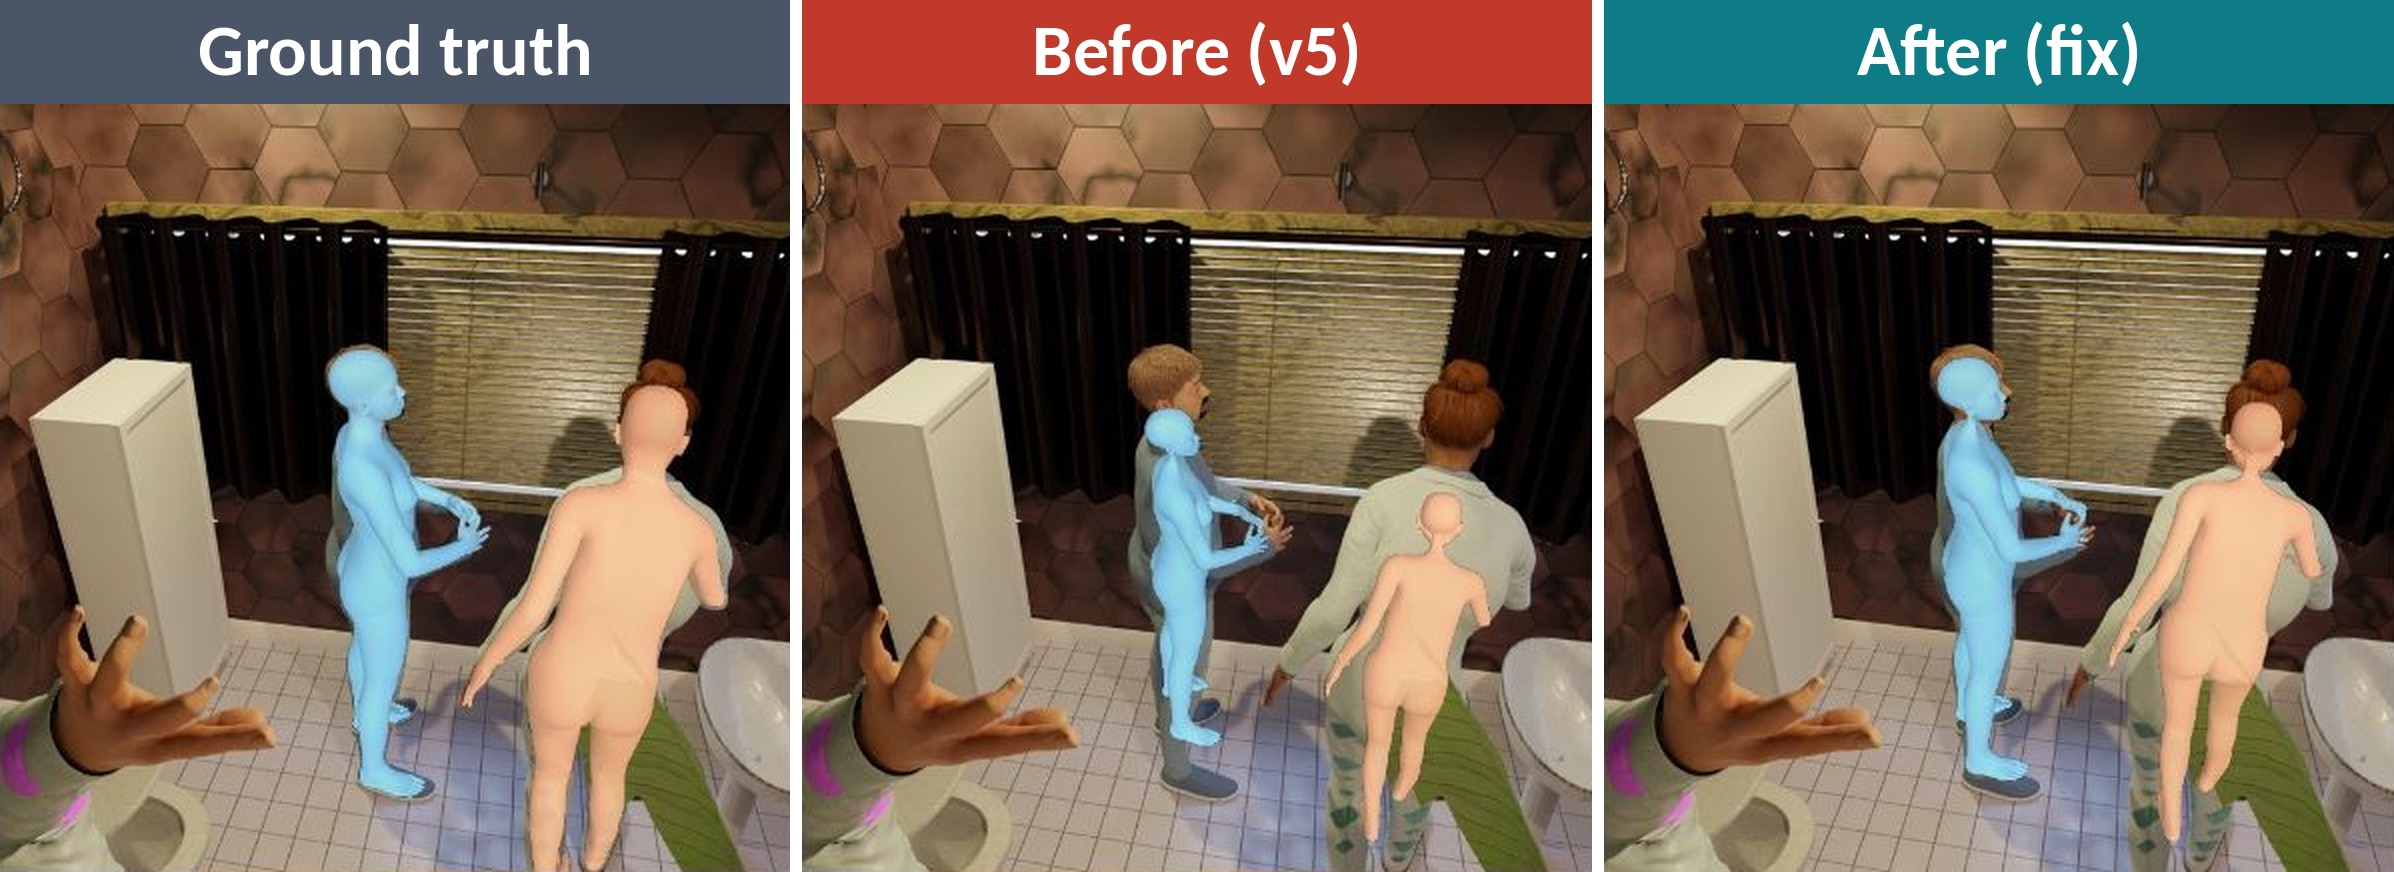
\includegraphics[width=\linewidth]{depth_before_after_579862}
\caption[Holdout image 579862 at the predicted depth: ground truth, Base, depth-fix pilot]{Holdout image 579862 rendered at each model's own predicted depth: ground truth, Base, and the depth-fix pilot (depth weight $\times$5, 10 epochs). The predicted body goes from 0.76 to 0.95 of its true height. Synthetic image; a good case, not a typical one.}
\label{fig:depth-579862}
\end{figure}
% F15 (also cited by Diagnostics 5.3; input it once, here or there)
% F15 Predicted against true root depth, AnnyOne holdout (100 images), Control and Final, setting V1 (eval, masked),
% each body at its own predicted depth. Generated from data/holdout_per_person_{control,final}.csv (rows with
% variant == V1_eval_masked: one row per matched person) by the scratchpad script thesis_plots/gen.py; numbers also in
% data/plot_stats.md. All points drawn, no subsampling (433 coordinates).
% Fit: least squares, pred = a * true + b (metres).
%   Control: n = 219 people (92 images), a = 0.276, b = 2.661 m, r = 0.46,
%            median |pred - true| = 1.237 m (mean 1.268), predicted too far for 99.1%,
%            mean root error 1402 mm (median 1312); fit meets identity at 3.67 m.
%   Final:   n = 214 people (89 images), a = 0.419, b = 1.746 m, r = 0.56,
%            median |pred - true| = 0.626 m (mean 0.654), predicted too far for 94.4%,
%            mean root error 728 mm (median 654); fit meets identity at 3.01 m.
%   Handover reference slopes: Final 0.42, Control 0.28, Base 0.33 (Base intercept 2.36 m). Final and Control agree
%   with the handover to two decimals. Base is not drawn: its per-person CSV has not arrived.
%   n is the number of matched people (detections), below the 222 ground-truth people of the 100 images.
% Needs: pgfplots (compat 1.18). Colours defined locally.
\definecolor{plFinal}{HTML}{2A78D6}% blue: Final
\definecolor{plControl}{HTML}{EB6834}% orange: Control
\definecolor{plBase}{HTML}{7A7A76}% grey: Base
\definecolor{plMasked}{HTML}{1BAF7A}% aqua: Final-masked
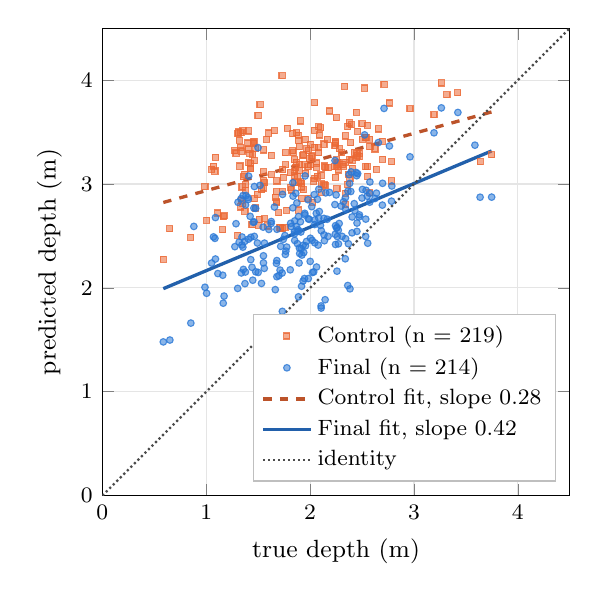
\begin{tikzpicture}
\begin{axis}[
  width=0.62\linewidth, height=0.62\linewidth,
  xlabel={true depth (m)}, ylabel={predicted depth (m)},
  xmin=0, xmax=4.5, ymin=0, ymax=4.5, axis equal image,
  xtick={0,1,...,4}, ytick={0,1,...,4},
  grid=major, grid style={gray!20},
  tick label style={font=\footnotesize}, label style={font=\small},
  legend style={font=\footnotesize, at={(0.97,0.03)}, anchor=south east, cells={anchor=west}, draw=gray!50},
  legend cell align=left,
]
% Control, n = 219
\addplot[only marks, mark=square*, mark size=1.1pt, color=plControl, fill opacity=0.55, draw opacity=0.8] coordinates {
(2.107,3.001) (2.404,3.231) (1.921,3.007) (1.070,3.171) (2.425,3.304) (1.849,3.015) (2.698,3.239) (1.862,3.159)
(3.748,3.283) (2.458,3.507) (3.637,3.213) (1.850,3.235) (1.956,3.103) (1.441,2.610) (1.353,2.811) (2.475,3.265)
(2.260,3.166) (2.023,2.824) (1.852,3.120) (1.287,3.298) (2.020,3.271) (1.767,3.185) (2.001,3.187) (1.918,2.972)
(2.384,3.054) (2.145,2.985) (2.696,3.411) (2.084,3.553) (1.991,3.242) (2.452,3.276) (2.369,3.093) (1.306,3.485)
(1.775,2.746) (1.711,2.579) (2.552,3.167) (1.742,3.064) (1.561,3.011) (1.897,3.361) (1.317,3.421) (1.762,3.303)
(1.089,3.256) (1.878,3.075) (1.477,2.770) (2.536,3.448) (2.245,3.395) (1.453,3.400) (2.363,2.995) (2.062,3.202)
(0.988,2.974) (2.242,3.412) (1.887,3.468) (1.939,3.281) (2.078,3.349) (1.603,3.491) (1.429,3.194) (2.451,3.291)
(2.044,3.355) (2.535,3.168) (2.173,3.157) (1.430,3.148) (1.373,2.736) (1.952,3.429) (1.421,3.296) (2.539,3.450)
(2.299,3.301) (2.138,3.173) (1.551,3.034) (1.004,2.652) (1.915,2.860) (1.911,3.022) (2.576,3.361) (2.322,3.171)
(1.932,3.274) (1.551,3.117) (1.834,3.322) (1.476,3.340) (1.325,3.173) (2.272,3.209) (1.983,3.322) (1.371,3.095)
(1.554,3.328) (1.867,3.209) (2.134,3.385) (2.472,3.298) (2.364,3.554) (2.040,3.516) (1.459,3.390) (1.355,3.513)
(2.106,3.086) (1.448,3.288) (2.245,3.064) (2.083,3.303) (1.625,3.278) (1.084,3.125) (2.100,3.542) (1.894,3.132)
(2.003,3.381) (1.052,3.143) (1.344,3.317) (2.255,3.234) (1.518,3.763) (1.404,3.511) (2.239,3.168) (2.108,2.922)
(1.463,2.860) (1.548,2.962) (2.405,3.153) (2.060,3.160) (1.949,3.187) (1.423,3.151) (2.342,3.208) (2.134,2.992)
(1.493,2.899) (1.681,3.030) (1.345,2.972) (2.150,3.159) (2.381,3.235) (2.639,3.141) (1.735,3.140) (1.464,3.225)
(2.308,3.188) (1.983,2.863) (1.676,2.927) (1.333,2.779) (1.338,2.845) (2.332,3.940) (1.730,4.042) (3.423,3.879)
(2.657,3.530) (2.240,3.369) (3.193,3.666) (2.764,3.780) (2.525,3.924) (2.962,3.726) (3.318,3.860) (3.264,3.973)
(2.712,3.959) (1.358,3.071) (1.310,3.500) (2.445,3.691) (2.500,3.581) (1.906,3.607) (1.626,3.088) (1.818,2.943)
(1.813,2.967) (1.980,3.165) (2.070,3.076) (2.550,3.567) (2.045,3.781) (1.559,2.665) (1.159,2.560) (2.187,3.703)
(1.782,3.538) (1.733,2.572) (1.377,2.939) (0.587,2.275) (2.259,2.956) (2.165,3.429) (1.172,2.694) (1.588,2.596)
(1.512,2.661) (0.650,2.569) (2.045,3.056) (1.680,2.828) (1.112,2.721) (1.852,3.079) (1.731,2.925) (1.461,3.412)
(1.889,3.011) (1.499,3.660) (2.449,3.254) (2.574,2.917) (2.376,3.588) (2.574,3.430) (1.401,3.395) (1.582,3.431)
(2.625,3.338) (2.395,3.571) (1.327,3.353) (1.809,3.108) (1.532,2.945) (1.276,3.321) (1.665,2.872) (1.407,3.334)
(1.888,2.749) (1.900,3.189) (0.852,2.487) (1.933,2.944) (1.966,3.339) (2.262,3.209) (2.035,3.029) (1.164,2.686)
(1.885,3.420) (2.342,2.911) (1.500,2.603) (1.836,3.300) (2.555,3.072) (2.340,3.463) (1.699,2.724) (1.334,3.495)
(2.392,3.396) (2.504,3.432) (1.834,3.486) (1.758,2.582) (2.787,3.213) (1.409,3.204) (1.717,2.577) (2.784,3.030)
(1.379,2.996) (2.339,2.803) (2.016,3.263) (1.303,2.508) (2.273,3.135) (1.680,2.821) (1.873,3.493) (2.280,3.339)
(2.089,3.472) (1.657,3.514) (2.251,3.640)
};
\addlegendentry{Control (n = 219)}
% Final, n = 214
\addplot[only marks, mark=*, mark size=1.2pt, color=plFinal, fill opacity=0.55, draw opacity=0.8] coordinates {
(2.107,1.806) (2.404,2.530) (1.921,2.316) (1.070,2.491) (2.425,2.811) (1.849,2.519) (2.698,3.007) (1.862,2.911)
(3.748,2.874) (2.458,3.100) (3.637,2.873) (1.956,2.405) (1.850,2.541) (1.441,2.198) (1.353,2.392) (2.475,2.703)
(2.260,2.582) (2.023,2.148) (1.852,2.457) (1.287,2.618) (2.020,2.458) (1.767,2.354) (2.001,2.255) (1.918,2.016)
(2.145,1.886) (2.384,1.991) (2.696,2.797) (2.431,2.744) (1.991,2.660) (2.084,2.950) (2.369,2.425) (2.452,2.624)
(1.306,2.824) (1.711,2.171) (1.775,2.393) (1.742,2.467) (1.561,2.431) (1.897,2.384) (1.317,2.441) (1.762,2.322)
(1.089,2.278) (1.878,2.426) (1.477,2.155) (2.536,2.662) (2.245,2.599) (1.453,2.631) (2.363,2.023) (2.062,2.201)
(0.988,2.006) (2.242,2.516) (1.887,2.545) (2.078,2.412) (1.939,2.340) (1.429,2.272) (1.603,2.563) (2.451,2.544)
(2.044,2.610) (2.535,2.495) (2.173,2.496) (1.430,2.487) (1.089,2.677) (1.373,2.041) (1.952,3.078) (2.539,2.939)
(2.299,2.788) (2.138,2.454) (1.551,2.309) (1.004,1.948) (1.915,2.378) (1.911,2.538) (2.576,3.020) (2.322,2.830)
(1.932,2.409) (1.551,2.241) (1.834,2.771) (1.476,2.766) (2.272,2.556) (1.983,2.665) (1.371,2.448) (1.867,2.591)
(2.134,2.669) (2.472,2.684) (2.364,2.931) (2.040,2.898) (1.355,2.889) (1.459,2.768) (1.946,2.090) (2.106,1.826)
(1.448,2.074) (2.245,2.418) (2.083,2.672) (1.625,2.620) (1.084,2.477) (0.881,2.592) (1.894,2.240) (2.100,2.602)
(2.003,2.478) (1.052,2.239) (1.344,2.413) (2.255,2.576) (1.949,2.703) (1.518,2.987) (1.404,2.851) (2.108,2.550)
(2.239,2.802) (1.463,2.496) (1.548,2.585) (2.405,2.683) (2.060,2.718) (1.949,2.718) (1.423,2.689) (2.134,2.511)
(2.342,2.759) (1.493,2.432) (1.681,2.564) (1.345,2.490) (2.639,2.912) (2.381,3.006) (2.150,2.915) (1.735,2.900)
(1.464,2.976) (2.308,2.496) (1.676,2.236) (1.983,2.090) (1.338,2.144) (3.423,3.689) (2.657,3.399) (3.193,3.493)
(2.240,3.226) (2.525,3.473) (3.587,3.374) (2.764,3.366) (2.962,3.262) (3.264,3.733) (2.712,3.728) (1.358,2.178)
(2.444,3.111) (2.500,2.865) (1.907,2.637) (1.626,2.639) (1.819,2.590) (1.813,2.622) (1.980,2.849) (2.071,2.853)
(2.550,2.883) (2.045,2.654) (1.559,2.188) (1.159,2.122) (2.187,2.919) (1.733,1.774) (1.377,2.153) (0.587,1.480)
(2.259,2.161) (2.165,2.661) (1.172,1.921) (1.512,1.700) (1.588,1.624) (0.650,1.498) (2.045,2.434) (1.680,2.263)
(1.112,2.138) (1.852,2.645) (1.731,2.143) (1.461,2.636) (1.889,2.687) (1.499,3.350) (2.574,2.825) (2.449,3.080)
(2.574,2.910) (2.376,3.090) (1.401,2.869) (2.625,2.861) (2.395,3.117) (1.809,2.174) (1.532,2.043) (1.276,2.397)
(1.665,1.983) (1.407,2.469) (1.888,1.914) (1.900,2.331) (0.852,1.661) (1.933,2.066) (1.966,2.447) (2.262,2.495)
(2.035,2.154) (1.885,2.560) (1.164,1.853) (2.342,2.474) (1.500,2.149) (1.836,2.883) (2.555,2.430) (2.340,2.868)
(1.699,2.118) (1.334,2.857) (2.392,2.928) (2.504,2.948) (1.834,3.012) (2.787,2.981) (1.758,2.504) (1.409,3.076)
(2.784,2.835) (1.717,2.400) (1.379,2.799) (2.339,2.280) (2.016,2.782) (1.303,1.995) (2.273,2.424) (1.680,2.108)
(1.873,2.818) (1.383,2.889) (2.280,2.620) (2.089,2.735) (2.251,2.895) (1.657,2.779)
};
\addlegendentry{Final (n = 214)}
\addplot[domain=0.587:3.748, samples=2, very thick, color=plControl!80!black, dashed] {0.2757*x + 2.6607};
\addlegendentry{Control fit, slope 0.28}
\addplot[domain=0.587:3.748, samples=2, very thick, color=plFinal!80!black] {0.4195*x + 1.7462};
\addlegendentry{Final fit, slope 0.42}
\addplot[domain=0:4.5, samples=2, densely dotted, thick, black!70] {x};
\addlegendentry{identity}
\end{axis}
\end{tikzpicture}


\section{Bone correction: zero-training, fine-tuned, final}
\label{sec:res-bone}
% absorbs draft main.tex lines 1006-1045 (only the four eliminations survive, as "what is not the cause", in Chapter 5; the LBS conclusion is deleted)
% needs: T9 (Diagnostics writer), F6, F9; girth 0.46 -> 1.00; head direction 19.1 (no training) -> 14.4 -> 13.1 (3579014:113; 3611336:200). Rules: "no sign of a PVE cost", never "PVE improved"; the correction "adds no parameters", "its origin is unknown"
\TODO{The correction without training, after a 2-epoch fine-tune, and in Final.}
% F6 (neck_before_after_v5.jpg) is placed in Chapter 5 (label fig:neck-before-after-v5); refer to it, do not place it twice.
% F9 (plan section 3; caption must say "fine-tuned 2 epochs with the fix", H 9). Office pair in Appendix D.
\begin{figure}[tbp]
\centering
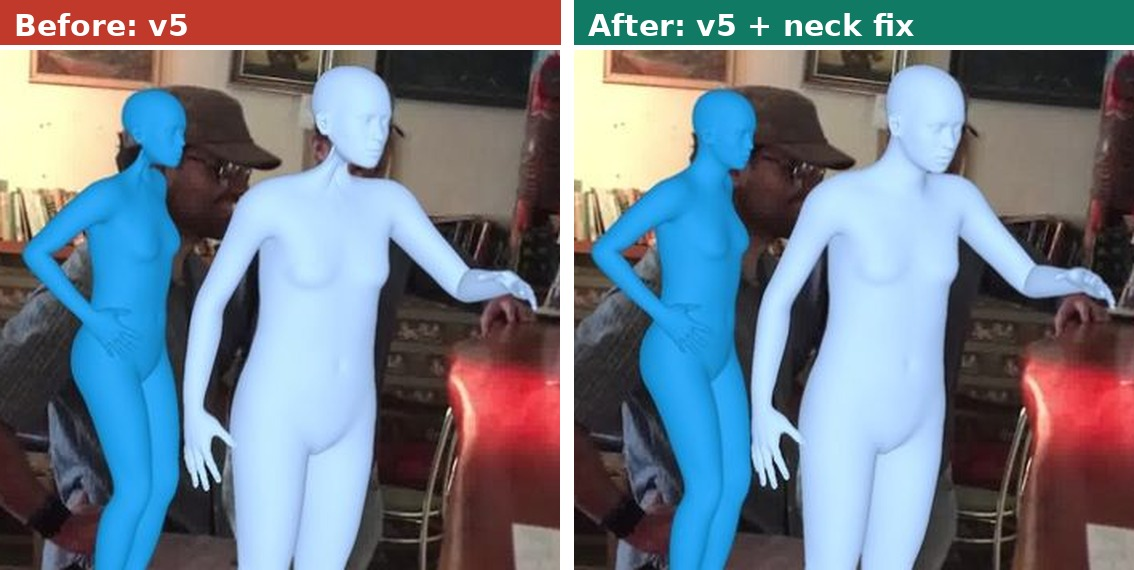
\includegraphics[width=0.85\linewidth]{neck_before_after_3dpw_bar}
\caption[3DPW test frame: Base vs bone correction with a 2-epoch fine-tune]{Real 3DPW test frame \texttt{downtown\_bar\_00} 701: Base next to the model fine-tuned for 2 epochs with the bone correction; bodies placed from the detector box; judged by eye, no metric. The two columns also differ by the fine-tune.}
\label{fig:neck-3dpw-bar}
\end{figure}

\section{Fingers}
\label{sec:res-fingers}
% absorbs - (new; draft line 946 claimed demos show neck elongation on all)
% needs: T10 (Diagnostics writer), F11 (pending); 17.3 -> 8.2 / 8.3 deg (3579014:114; 3611336:201). Rule: "predicted fingers have not been shown on a real photo" until F11 exists
\TODO{Finger angles before and after the correction; no real-photo render yet.}
% F11: cluster demo with --relax_hands 0 (plan section 3 command)
\begin{figure}[tbp]
\centering
\fbox{\parbox[c][3cm][c]{0.8\linewidth}{\centering\TODO{F11 pending: cluster demo with -{}-relax\_hands 0 (plan section 3 command)}}}
\caption{Predicted fingers on the 12 demo images, Final with predicted (not rest-pose) fingers next to Base.}
\label{fig:fingers-demo}
\end{figure}

\section{Final model vs Control vs Base on AnnyOne}
\label{sec:res-final}
% absorbs draft main.tex lines 665-694 (the 145 -> 73.6 -> 74.3 history moves to Section~\ref{sec:res-history} as a V0 table)
% needs: T15 part A, F12 (pending), F20; 73.7 / 50.3 / 87.0 vs 77.4 / 56.4 / 89.0 vs 70.5 / 53.3 / 90.2 (H 5/7); what is inside noise (PVE -3.7) and what is not (PA-PVE -6.1, root -48%); recall cost -2 / -3.2
\TODO{The full V1 table and its reading against the noise floor.}
% T15 Final model vs Control vs Base (Results 6.5-6.6). Owner: Results writer.
% Source: REWRITE_PLAN.md section 4 (T15); H 5/7 table; H 0b 3DPW table.
% Part A: 3570222:40 (Base), long_pc_dist5 = 3572482 (depth pilot, x5, 10 epochs), exp6 fine-tune = 3579014
% (neck pilot), 3611339:182-198 (Control), 3611336:191-207 (Final).
% Part B: 3612073 (Base), 3612074 (Mixed-L old labels = v9 e62), 3612075 (neck pilot), 3611339:215-220,
% 3611336:224-229, 3614192 (NAVER); lines :117-124 for the 3612073-5 jobs.
% Old-label 3DPW numbers (119.1 / 102.5 / 111.5) are retired and never appear next to these.
\begin{table}[tbp]
\centering\footnotesize
\setlength{\tabcolsep}{3pt}
\begin{subtable}{\linewidth}
\centering
\begin{tabular}{@{}lrrrrr@{}}
\toprule
 & Base & \shortstack[r]{Depth\\pilot} & \shortstack[r]{Neck\\pilot} & Control & Final \\
\midrule
PVE (mm) & \BasePVE & 74.8 & 68.8 & \ControlPVE & \FinalPVE \\
PA-PVE (mm) & \BasePAPVE & 54.0 & 50.9 & \ControlPAPVE & \textbf{\FinalPAPVE} \\
Recall (\%) & \BaseRecall & 87.8 & 89.4 & \ControlRecall & \FinalRecall \\
Root error (mm) & \BaseRootErr & \DepthPilotRootErr & 1429 & \ControlRootErr & \textbf{\FinalRootErr} \\
Depth slope & \BaseSlope & 0.38 & 0.34 & \ControlSlope & \FinalSlope \\
Depth intercept (m) & \BaseIntercept & 1.59 & 2.56 & \ControlIntercept & \FinalIntercept \\
Size ratio & \BaseSize & 0.84 & 0.58 & \ControlSize & \FinalSize \\
Neck girth pred/GT & \BaseGirth & 0.457 & 0.997 & \ControlGirth & \FinalGirth \\
PVE\textsubscript{neck} (mm) & 27.3 & 27.7 & 10.7 & \ControlNeckSkin & \FinalNeckSkin \\
Global head direction (deg) & \BaseHeadDir & 12.7 & \NeckPilotHeadDir & \ControlHeadDir & \FinalHeadDir \\
Fingers (deg) & \BaseFingers & 17.4 & 8.3 & \ControlFingers & \FinalFingers \\
neck02 bone (deg) & \BaseNeckTwo & 175.5 & 4.7 & \ControlNeckTwo & \FinalNeckTwo \\
head bone (deg) & 177.9 & 178.0 & 11.2 & \ControlHeadBone & \FinalHeadBone \\
\bottomrule
\end{tabular}
\caption{AnnyOne holdout, 100 images, setting V1 (helper bones masked, matched people); root error, depth fit and size ratio with each body at the model's own predicted depth.}
\label{tab:final-annyone}
\end{subtable}

\vspace{1em}
\begin{subtable}{\linewidth}
\centering
\begin{tabular}{@{}lrrrrrr@{}}
\toprule
 & Base & Mixed-L & \shortstack[r]{Neck\\pilot} & Control & Final & \shortstack[r]{Multi-HMR-\\Anny} \\
\midrule
PVE (mm) & \BaseThreeDPW & \BaseOldThreeDPW & \NeckPilotThreeDPW & \ControlThreeDPW & \textbf{\FinalThreeDPW} & \NAVERThreeDPW \\
PA-PVE (mm) & \BasePAThreeDPW & \BaseOldPAThreeDPW & 68.7 & \ControlPAThreeDPW & \textbf{\FinalPAThreeDPW} & \NAVERPAThreeDPW \\
MPJPE (mm)$^{b}$ & 126.9 & 94.8 & 124.8 & \ControlMPJPEThreeDPW & \textbf{\FinalMPJPEThreeDPW} & \NAVERMPJPEThreeDPW \\
Precision (\%) & \BasePrecThreeDPW & \BaseOldPrecThreeDPW & 53 & 62 & \FinalPrecThreeDPW & \NAVERPrecThreeDPW \\
Recall (\%) & 100 & \BaseOldRecallThreeDPW & 100 & 99 & \FinalRecallThreeDPW & \NAVERRecallThreeDPW \\
\addlinespace
AnnyOne test-100 PVE$^{c}$ & \BaseVzeroPVE & \BaseOldVzeroPVE & 72.7 & 81.2 & \FinalTestHundredPVE & (\NAVERAnnyOne)$^{a}$ \\
\bottomrule
\end{tabular}
\caption{3DPW test, corrected (v23) labels, all 8,190 images, setting V0, same evaluation script for every model. Mixed-L was trained on the labels before their correction and is tested on the corrected ones, like every model here.}
\label{tab:final-3dpw}
\end{subtable}
\caption[Final against Control and Base on the AnnyOne holdout and the 3DPW test]{Final against its Control and against Base. One run per model, no seed; two identical runs differed
by \NoisePVE\,mm PVE, so the PVE gap between Control and Final (\ControlPVE{} vs \FinalPVE) is within run-to-run
variation, while PA-PVE, root error, neck and fingers are not. Depth pilot: depth fix, depth weight $\times$5, 10 epochs;
neck pilot: bone correction and a 2-epoch fine-tune. 3DPW numbers are against our converted labels and are not
comparable with published 3DPW results. $^{a}$Multi-HMR-Anny masks the helper bones by design, so its number is V1 and
compares with Final's \FinalPVE{} in (a); it was most likely trained on these 100 images. $^{b}$Mean over all 163 Anny
joints, pelvis-centred. $^{c}$The same 100 images as (a) in setting V0 (helper bones unmasked).}
\label{tab:final}
\end{table}

% F20 In-training PVE per epoch, Final and Control, epochs 1-10 (one run each, no seed).
% Left: 3DPW-Anny validation (300 images, corrected v23 labels). Right: AnnyOne holdout as evaluated during training
% (setting V0, as train.py prints it; NOT the V1 trace numbers 73.7 / 77.4 mm).
% Data: data/val_curves_exp7.csv (columns final_3dpwval_pve, control_3dpwval_pve, final_holdout_pve,
% control_holdout_pve), written inline; all 40 values drawn. Generated by the scratchpad script thesis_plots/gen.py.
%   3DPW val, Final:   min 73.4 (epoch 7), last 74.5, mean over epochs 75.69
%   3DPW val, Control: min 75.5 (epoch 4), last 75.9, mean over epochs 77.72
%   holdout V0, Final:   min 78.9 (epoch 9), last 79.3, mean over epochs 80.73
%   holdout V0, Control: min 76.8 (epoch 9), last 81.2, mean over epochs 79.19
% Needs: pgfplots (compat 1.18) with \usepgfplotslibrary{groupplots}. Colours defined locally.
\definecolor{plFinal}{HTML}{2A78D6}% blue: Final
\definecolor{plControl}{HTML}{EB6834}% orange: Control
\definecolor{plBase}{HTML}{7A7A76}% grey: Base
\definecolor{plMasked}{HTML}{1BAF7A}% aqua: Final-masked
\begin{tikzpicture}
\begin{groupplot}[
  group style={group size=2 by 1, horizontal sep=1.6cm},
  width=0.5\linewidth, height=5cm,
  xmin=0.5, xmax=10.5, xtick={1,...,10}, xlabel={epoch},
  ylabel={PVE (mm)},
  grid=major, grid style={gray!20},
  tick label style={font=\footnotesize}, label style={font=\small}, title style={font=\small},
]
\nextgroupplot[title={3DPW validation}, ymin=72, ymax=84,
  legend style={font=\footnotesize, at={(0.97,0.97)}, anchor=north east, draw=gray!50}, legend cell align=left]
\addplot[color=plControl, mark=square*, mark size=1.6pt, thick, dashed, mark options={solid}] coordinates {(1,80.6) (2,76.1) (3,80.9) (4,75.5) (5,77.2) (6,78.2) (7,77.4) (8,76.7) (9,78.7) (10,75.9)};
\addlegendentry{Control}
\addplot[color=plFinal, mark=*, mark size=1.7pt, thick] coordinates {(1,79.9) (2,75.7) (3,77.8) (4,74.4) (5,75.5) (6,75.0) (7,73.4) (8,75.4) (9,75.3) (10,74.5)};
\addlegendentry{Final}
\nextgroupplot[title={AnnyOne holdout (in training)}, ymin=72, ymax=84]
\addplot[color=plControl, mark=square*, mark size=1.6pt, thick, dashed, mark options={solid}] coordinates {(1,79.3) (2,77.7) (3,77.7) (4,79.8) (5,79.4) (6,78.2) (7,83.2) (8,78.6) (9,76.8) (10,81.2)};
\addplot[color=plFinal, mark=*, mark size=1.7pt, thick] coordinates {(1,81.1) (2,80.2) (3,80.1) (4,80.8) (5,81.6) (6,82.3) (7,81.1) (8,81.9) (9,78.9) (10,79.3)};
\end{groupplot}
\end{tikzpicture}

% F12: trace panels stacked on the cluster (plan section 3 command)
\begin{figure}[tbp]
\centering
\fbox{\parbox[c][3cm][c]{0.8\linewidth}{\centering\TODO{F12 pending: trace panels stacked on the cluster (plan section 3 command)}}}
\caption{Six holdout images: photo, ground truth, Base, Final, each at its own predicted depth.}
\label{fig:holdout-montage}
\end{figure}

\section{3DPW test on the corrected labels}
\label{sec:res-3dpw}
% absorbs draft main.tex lines 1131-1221 (old-label numbers retired; validation-trajectory text moves to history)
% needs: T15 part B, F10 (pending); 121.8 / 95.5 / 120.2 / 91.5 / 89.0 (3612073-5; 3611339; 3611336); most of the gain is training on 3DPW (Control 91.5); the fixes add 2.5 mm; precision 64% explained (bystanders not labelled). Wording: "lowest error on our 3DPW-Anny labels", "not comparable with published 3DPW numbers"
\TODO{Every model on the v23 test labels with the same script.}
% F10 (plan section 3): demo job 3612078 montages, each photo | Base | photo | Final, labels baked in
% (data/CLUSTER_ANSWERS.md). 3 of the 8 3DPW frames received; missing: downtown_bar, downtown_walking,
% downtown_sitOnStairs, downtown_walkBridge, weekly market.
\begin{figure}[tbp]
\centering
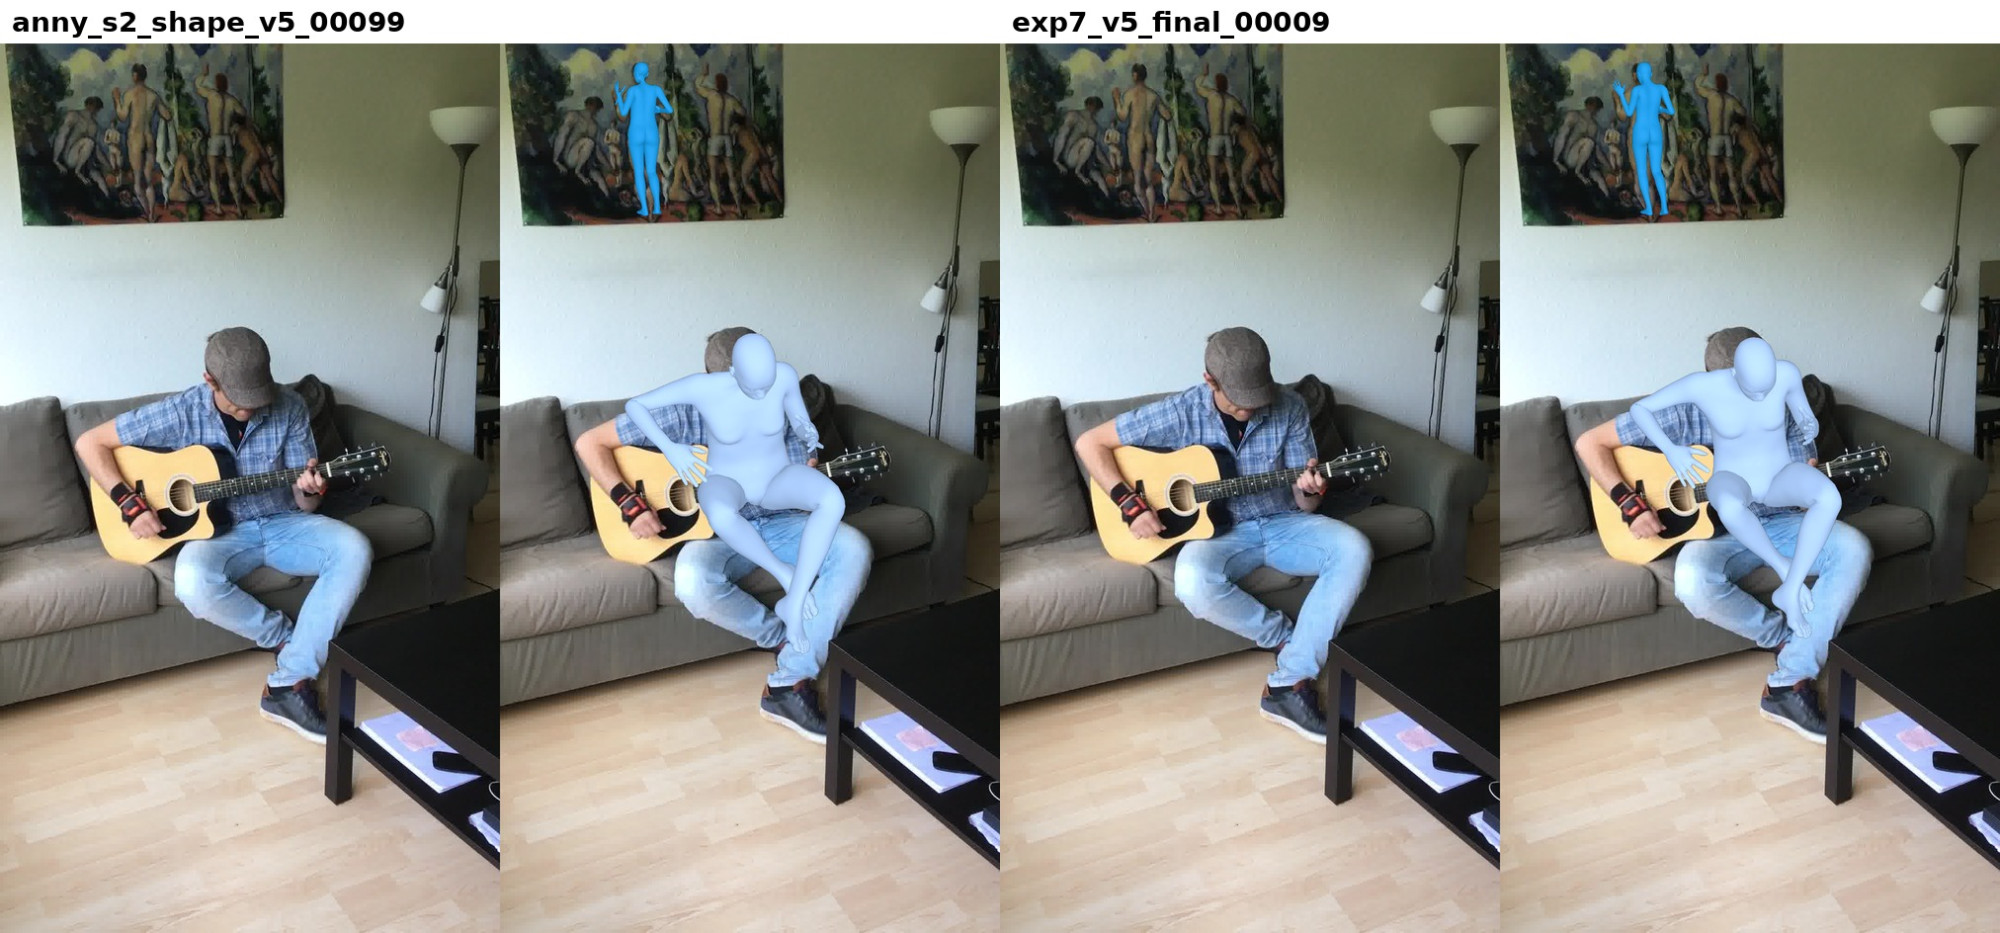
\includegraphics[width=\linewidth]{F10_3dpw_guitar_v5_vs_final}\\[2pt]
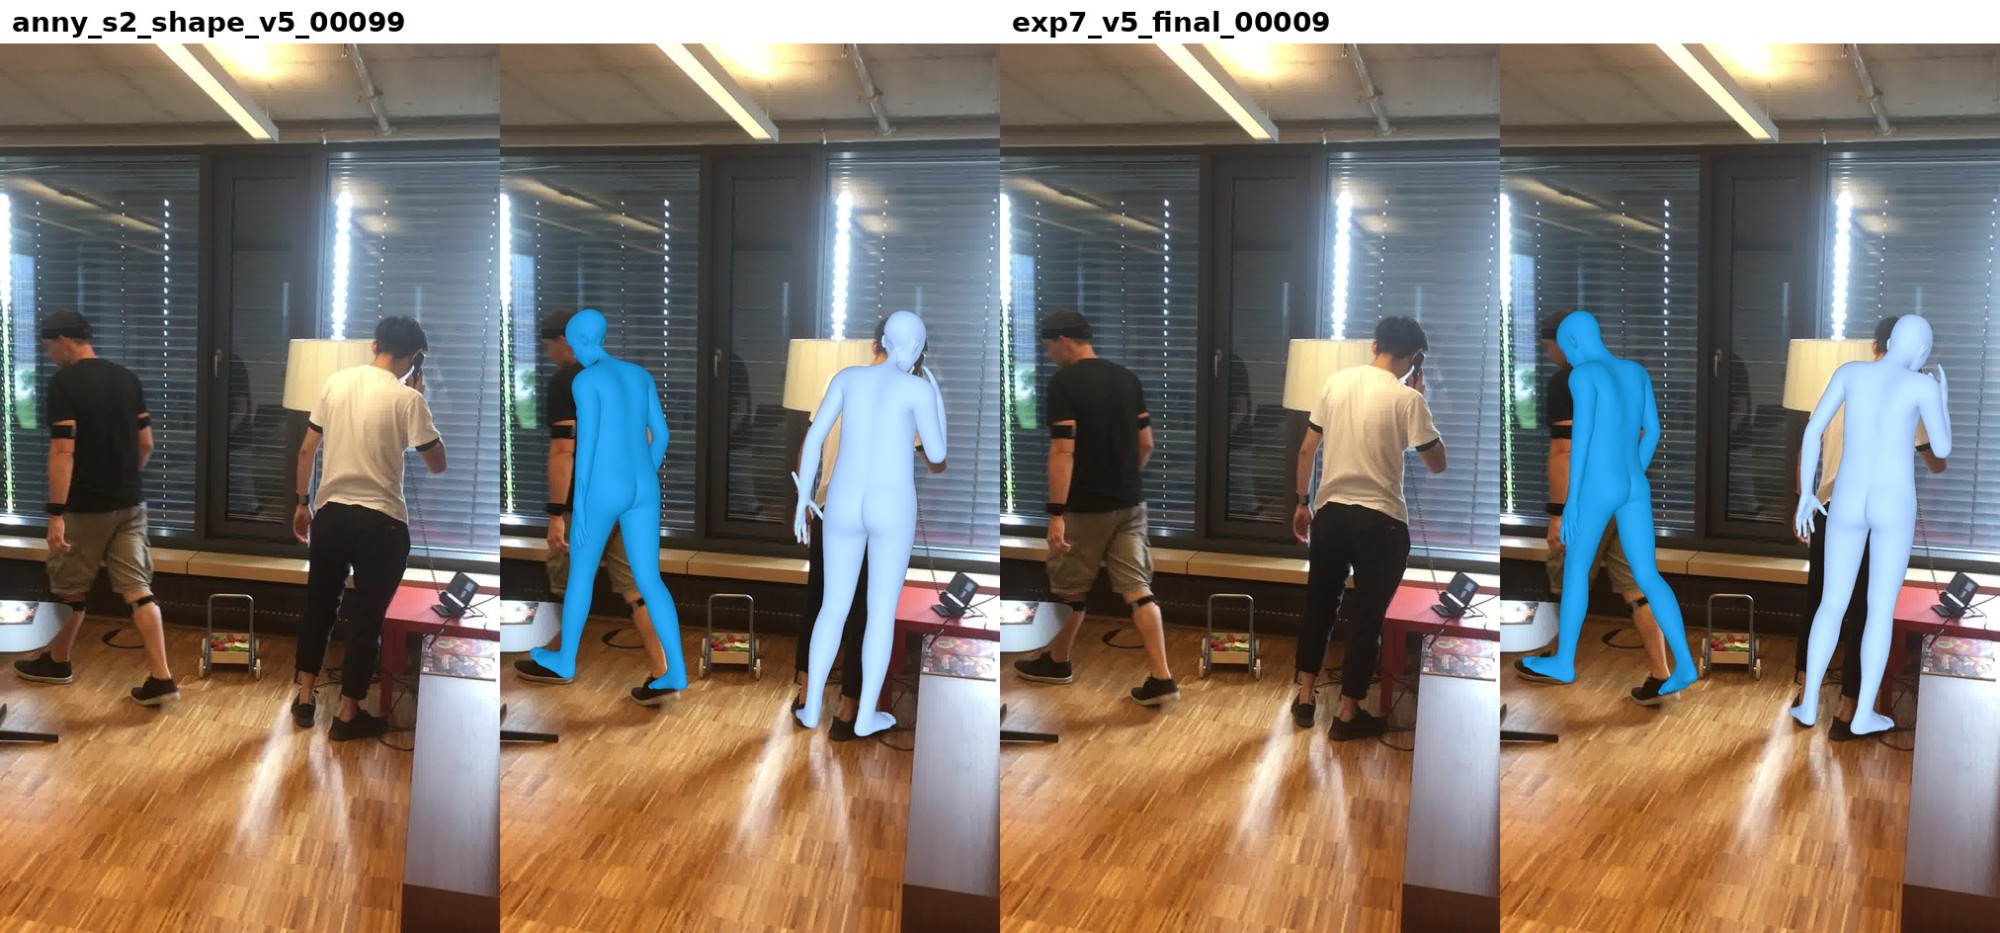
\includegraphics[width=\linewidth]{F10_3dpw_office_v5_vs_final}\\[2pt]
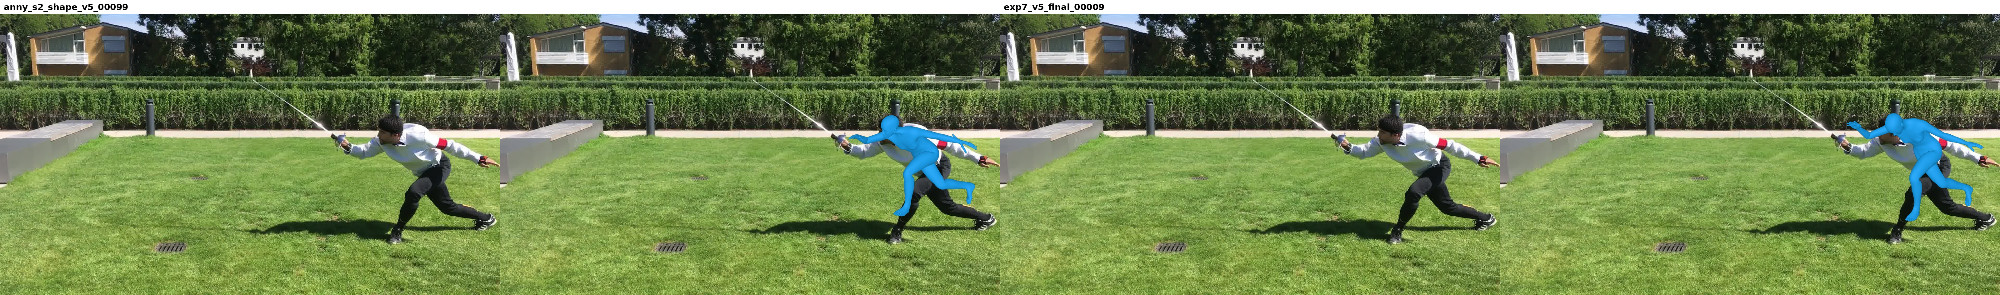
\includegraphics[width=\linewidth]{F10_3dpw_fencing_v5_vs_final}
\caption[3DPW test frames, Base vs Final]{3DPW test frames, each shown as photo and Base, then photo and Final; bodies placed from the detector box; judged by eye, no metric. \TODO{five more frames pending}}
\label{fig:3dpw-overlays}
\end{figure}

\section{Real photos: Relative Human and the demo}
\label{sec:res-rh}
% absorbs - (new)
% needs: T12, F13, F16, F17 (pending); gender 46.5 -> 64.2; AUC 0.61 -> 0.72; babies 0.44 vs adults 0.54; recall 47 -> 65; by-eye reading of the 12 images. Rule: children "a measured improvement, not solved"; never convert Anny ages to years
\TODO{Relative Human numbers and the by-eye reading of the demo images.}
% T12 Relative Human (Results 6.7 / 6.8). Owner: Results writer.
% Source: REWRITE_PLAN.md section 4 (T12); H 0a "DECIDED"; H 0b; H 3.4.
% Base = 3611285_0 (:23-31), Final = 3612131 (:25-33), Final-masked = 3613616 (logs/eval_rh_3613616_0.out).
% Demo spread: jobs 3612078 (Final) vs 3613617 (Final-masked), 12 images, [shape] lines (H 0a).
% "--" = not reported in the sources.
\begin{table}[tbp]
\centering\small
\begin{tabular}{@{}lrrr@{}}
\toprule
 & Base & Final & Final-masked \\
\midrule
Recall (\%) & \RHRecallBase & \RHRecallFinal & \RHRecallMasked \\
Gender accuracy (\%) & \RHGenderBase & \RHGenderFinal & \RHGenderMasked \\
\quad mean gender, men (male = 0) & 0.535 & 0.551 & 0.717 \\
\quad mean gender, women (female = 1) & 0.551 & 0.861 & 0.860 \\
Child-vs-adult AUC & \RHAUCBase & \RHAUCFinal & \RHAUCMasked \\
\addlinespace
Mean age, adult & 0.631 & 0.536 & 0.638 \\
\quad teen & 0.597 & 0.524 & -- \\
\quad kid & 0.613 & 0.500 & 0.611 \\
\quad baby & 0.624 & 0.438 & 0.524 \\
Babies with age $<$ 0.45 (\%) & 2.6 & 49.3 & 16.9 \\
Mean height, adult & 0.507 & 0.500 & -- \\
\quad kid & 0.451 & 0.466 & -- \\
\quad baby & 0.394 & 0.464 & -- \\
Matched children + adults & 948 & 1,305 & -- \\
\midrule
\multicolumn{4}{@{}l}{\emph{Demo images: standard deviation of the prediction}} \\
Muscle & -- & 0.04 & 0.06 \\
Weight & -- & 0.04 & 0.11 \\
Cup size & -- & 0.05 & 0.11 \\
Firmness & -- & 0.04 & 0.11 \\
Age & -- & 0.03 & 0.08 \\
\bottomrule
\end{tabular}
\caption{Body shape on real photos. Upper part: Relative Human validation split (635 images, 2,130 labelled people),
detected people only, matched to the labelled boxes at IoU $\geq$ 0.3; ``child'' means a predicted age below 0.45;
the matched sets differ between models because recall differs. Lower part: spread of the predicted phenotypes over all
detected people of the 12 demo images (4 photos and 8 3DPW test frames), not matched to people. The neck pilot
(bone correction and a 2-epoch fine-tune) is the same as Base within run-to-run variation (AUC 0.613).}
\label{tab:relhuman}
\end{table}

% F13 (plan section 3). Source docs/figures/final_model_real_photos.jpg (labels baked in).
\begin{figure}[tbp]
\centering
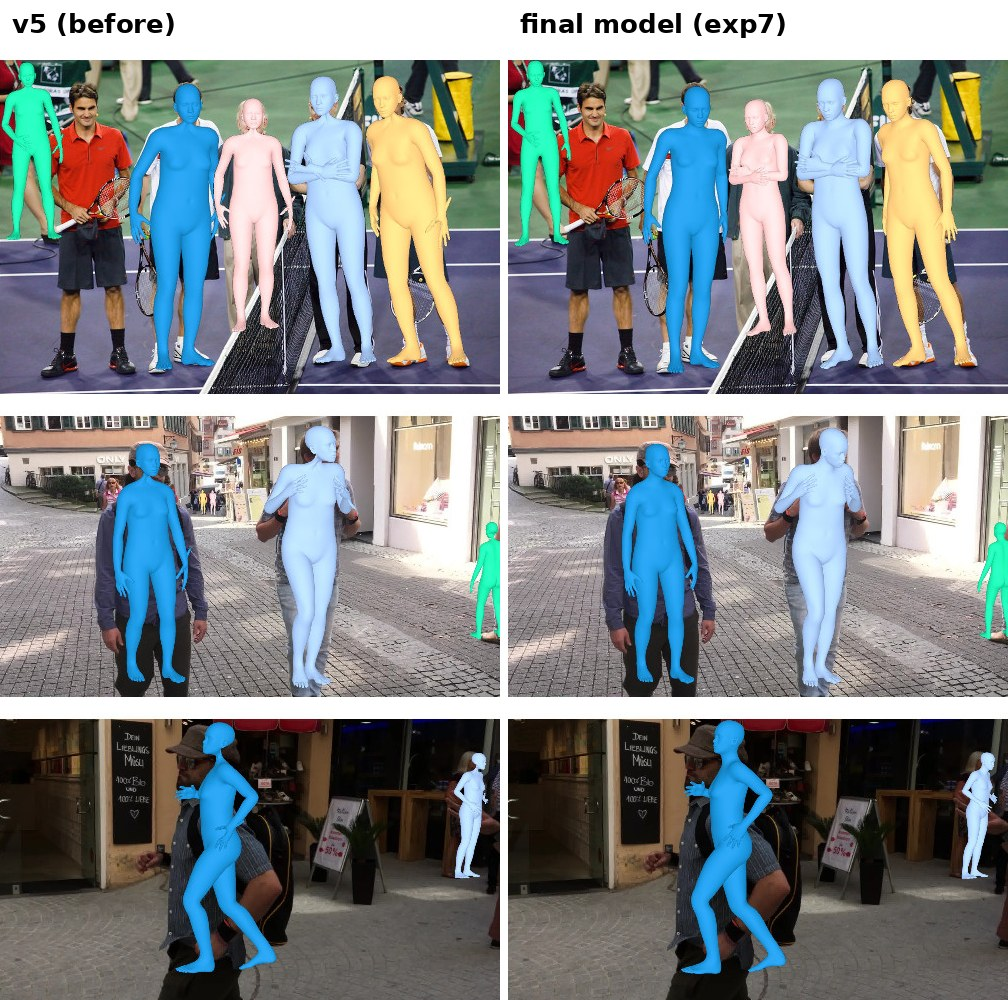
\includegraphics[width=0.8\linewidth]{final_model_real_photos}
\caption[Three real photos, Base vs Final]{Three real photos, Base (left) and Final (right), bodies placed from the detector box: most men get male bodies, women stay female, the boy stays an adult body. Judged by eye; no metric exists for these images.}
\label{fig:real-photos}
\end{figure}
% F16 Predicted Anny age per Relative Human group (adult, teen, kid, baby) for Base and Final, with the child
% threshold 0.45 (Results 6.7). PLACEHOLDER: data pending.
% Waits for (REWRITE_PLAN.md section 3 "F15 and F16, CSVs"; section 7 Q11):
%   data/F16_rh_base.csv    <- results/diagnostics/relative_human_val_anny_s2_shape_v5_00099/per_person.csv
%   data/F16_rh_final.csv   <- results/diagnostics/relative_human_val_exp7_v5_final_00009/per_person.csv
%   data/F16_rh_masked.csv  <- the masked arm's per_person.csv (optional third model)
% Column names known (data/CLUSTER_ANSWERS.md): age_group, pred_age, matched (keep matched rows).
% Then one \addplot[boxplot] table[y=pred_age] per age_group and model (pgfplots statistics library is loaded).
\begin{figure}[tbp]
\centering
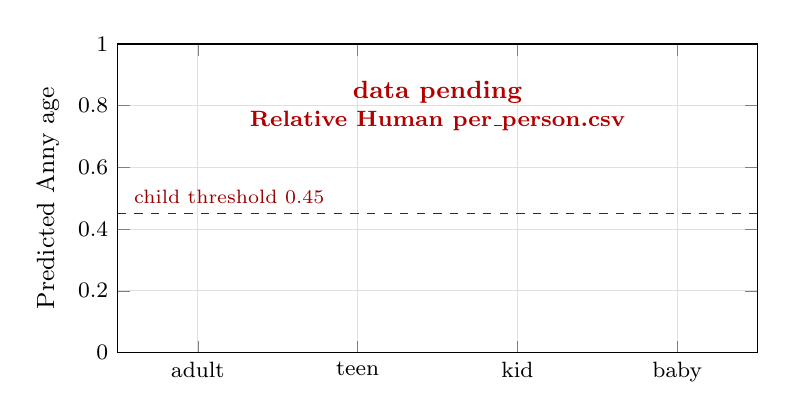
\begin{tikzpicture}
\begin{axis}[
  width=0.8\linewidth, height=5.5cm,
  ylabel={Predicted Anny age}, ymin=0, ymax=1,
  xmin=0.5, xmax=4.5, xtick={1,2,3,4}, xticklabels={adult, teen, kid, baby},
  grid=major, grid style={gray!25},
  tick label style={font=\footnotesize}, label style={font=\small},
]
\draw[dashed, red!60!black] (axis cs:0.5,0.45) -- (axis cs:4.5,0.45) node[pos=0.01, anchor=south west, font=\scriptsize] {child threshold 0.45};
\node[font=\small\bfseries, red!70!black, align=center] at (axis cs:2.5,0.8) {data pending\\[-1pt]\footnotesize Relative Human per\_person.csv};
\end{axis}
\end{tikzpicture}
\caption{Predicted Anny age per Relative Human age group, Base and Final; detected people only. \TODO{plot pending:
Relative Human per-person CSVs}}
\label{fig:rh-age}
\end{figure}

% F17: cluster demo with --rest_pose 1 (plan section 3 command)
\begin{figure}[tbp]
\centering
\fbox{\parbox[c][3cm][c]{0.8\linewidth}{\centering\TODO{F17 pending: cluster demo with -{}-rest\_pose 1 (plan section 3 command)}}}
\caption{Rest-pose line-up: every detected person of the 12 demo images in rest pose, Final, so only body shape differs.}
\label{fig:rest-lineup}
\end{figure}

\section{The shape-mask trade-off}
\label{sec:res-mask}
% absorbs - (new)
% needs: T12 (masked column and demo spread); variety back (std 0.04 -> 0.11) vs gender back to 49.3% and children weaker; the decision (H 0a "DECIDED"); the partial mask (pending, Final-masked-7)
\TODO{Final-masked against Final: shape variety against gender and children.}

\section{Baseline comparison and model cost}
\label{sec:res-baseline}
% absorbs draft main.tex lines 631-652 (paper table replaced by the measured Multi-HMR-Anny row)
% needs: T16, F18; 60.3 / 126.9 vs 73.7 / 89.0; cost measured: NAVER 380.94 M (head 76.57 M), backbone 1917.2 GFLOPs, ms not measurable for its class; Final 318.38 M, 1927.4 GFLOPs, 77.9 ms (A100) / 110 ms (A40). Fixed wording on the in-sample 60.3 (plan section 5)
\TODO{Multi-HMR-Anny against Final on both sets, with the in-sample caveat; parameters, FLOPs and time.}
% Source macros retain the measured results and provenance in numbers_results.tex.
% Split the former 12-column table for readable reconstruction/cost comparisons.
\begin{table}[!tbp]
\centering\small
\setlength{\tabcolsep}{3pt}
\begin{tabular}{@{}lrrrrrrc@{}}
\toprule
& \multicolumn{3}{c}{AnnyOne holdout (V1)} & \multicolumn{3}{c}{3DPW test (v23)} & \\
\cmidrule(lr){2-4}\cmidrule(lr){5-7}
Model & PVE & PA-PVE & Recall & PVE & PA-PVE & Recall & \shortstack{3DPW\\training} \\
\midrule
Released baseline & \NAVERAnnyOne$^a$ & \NAVERPAAnnyOne$^a$ & \NAVERRecallAnnyOne$^a$ & \NAVERThreeDPW & \NAVERPAThreeDPW & \NAVERRecallThreeDPW & no \\
Teacher (Final) & \FinalPVE & \FinalPAPVE & \FinalRecall & \textbf{\FinalThreeDPW} & \textbf{\FinalPAThreeDPW} & \FinalRecallThreeDPW & yes \\
Student (ViT-B) & \StudentPVE & \StudentPAPVE & \StudentRecall & \StudentThreeDPW & \StudentPAThreeDPW & \StudentRecallThreeDPW & yes \\
Control & \ControlPVE & \ControlPAPVE & \ControlRecall & \ControlThreeDPW & \ControlPAThreeDPW & 99 & yes \\
Base & \BasePVE & \BasePAPVE & \BaseRecall & \BaseThreeDPW & \BasePAThreeDPW & 100 & no \\
\bottomrule
\end{tabular}
\caption[Reconstruction comparison of student and reference models]{Reconstruction comparison. Errors are in mm;
recall is in percent. One checkpoint is evaluated per model; thesis-trained models were not repeated across seeds. 3DPW errors use converted Anny labels and are not
comparable with published SMPL-space results. $^a$The released baseline was trained on the AnnyOne release,
which includes these holdout images, so its synthetic result is potentially in-sample. The real-image
training exposure differs between released baseline and student/teacher.}
\label{tab:baseline}
\end{table}

\begin{table}[!tbp]
\centering\small
\begin{tabular}{@{}lrrrr@{}}
\toprule
Model & Params (M) & GFLOPs & \shortstack{Latency\\L40S (ms)} & \shortstack{Latency\\A100 (ms)} \\
\midrule
Released baseline & \NAVERParams & $\geq$\NAVERBackboneGFLOPs$^b$ & n/m & n/m \\
Teacher (Final) & \FinalParams & \FinalGFLOPs & \TeacherMsLFortyS & \TeacherMsAHundred \\
Student (ViT-B) & \StudentParams & \StudentGFLOPs & \StudentMsLFortyS & n/m \\
\bottomrule
\end{tabular}
\caption[Model size, computation and recorded forward latency]{Model cost at 672\,px input and one person.
One multiply-add counts as two FLOPs. Latency is median batch-one forward time in fp32 with TF32; compare
only within a GPU column. The student/teacher L40S pair was measured in the same job. n/m: not measured.
$^b$The baseline figure counts only its backbone, so total computation is higher. Base and Control share
the teacher architecture; fixed rotation corrections add no trainable parameters.}
\label{tab:model-cost}
\end{table}

% F18 Parameters and GFLOPs against 3DPW-test PVE (Results 6.9). Owner: Results writer.
% Numbers from tables/T16 via numbers_results.tex: NAVER 380.94 M / >= 1917.2 GFLOPs (backbone only,
% head FLOPs not countable for its class; job 3614947) / 126.9 mm; Final 318.38 M / 1927.4 / 89.0 mm;
% Student 101.38 M / 603.3 GFLOPs, PVE pending (job 3614191): drawn as a dashed vertical line until known.
% 19 Oct: the Student's measured point (110.1 mm, job 3614191) replaces the dashed line.
\begin{figure}[!tbp]
\centering
\begin{tikzpicture}
\begin{groupplot}[
  group style={group size=2 by 1, horizontal sep=0.6cm, y descriptions at=edge left},
  width=0.5\linewidth, height=4.8cm,
  ylabel={3DPW test PVE (mm)}, ymin=70, ymax=140,
  grid=major, grid style={gray!25},
  tick label style={font=\footnotesize}, label style={font=\small},
]
\nextgroupplot[xlabel={Parameters (M)}, xmin=0, xmax=450]
  \draw[densely dotted, black!60] (axis cs:0,\BarThreeDPW) -- (axis cs:450,\BarThreeDPW);
  \node[font=\scriptsize, anchor=south east, black!70] at (axis cs:445,\BarThreeDPW) {95\,\% bar};
  \addplot[only marks, mark=square*, color=gray!70!black] coordinates {(\NAVERParams,\NAVERThreeDPW)};
  \node[font=\scriptsize, anchor=north east] at (axis cs:\NAVERParams,\NAVERThreeDPW-2) {Multi-HMR-Anny};
  \addplot[only marks, mark=*, color=blue!70!black] coordinates {(\FinalParams,\FinalThreeDPW)};
  \node[font=\scriptsize, anchor=north, blue!70!black] at (axis cs:\FinalParams,\FinalThreeDPW-2) {Teacher};
  \addplot[only marks, mark=triangle*, mark size=2.5pt, color=red!70!black] coordinates {(\StudentParams,\StudentThreeDPW)};
  \node[font=\scriptsize, anchor=south, red!70!black] at (axis cs:\StudentParams,\StudentThreeDPW+2) {Student};
\nextgroupplot[xlabel={GFLOPs}, xmin=0, xmax=2400]
  \draw[densely dotted, black!60] (axis cs:0,\BarThreeDPW) -- (axis cs:2400,\BarThreeDPW);
  \addplot[only marks, mark=square*, color=gray!70!black] coordinates {(\NAVERBackboneGFLOPs,\NAVERThreeDPW)};
  \draw[->, gray!70!black] (axis cs:\NAVERBackboneGFLOPs,\NAVERThreeDPW) -- (axis cs:\NAVERBackboneGFLOPs+300,\NAVERThreeDPW);
  \node[font=\scriptsize, anchor=north east, align=right] at (axis cs:\NAVERBackboneGFLOPs+250,\NAVERThreeDPW-2) {Multi-HMR-Anny\\(backbone only)};
  \addplot[only marks, mark=*, color=blue!70!black] coordinates {(\FinalGFLOPs,\FinalThreeDPW)};
  \node[font=\scriptsize, anchor=north, blue!70!black] at (axis cs:\FinalGFLOPs,\FinalThreeDPW-2) {Teacher};
  \addplot[only marks, mark=triangle*, mark size=2.5pt, color=red!70!black] coordinates {(\StudentGFLOPs,\StudentThreeDPW)};
  \node[font=\scriptsize, anchor=south, red!70!black] at (axis cs:\StudentGFLOPs,\StudentThreeDPW+2) {Student};
\end{groupplot}
\end{tikzpicture}
\caption[Model size and compute against 3DPW-test PVE]{Model size and compute against 3DPW-test PVE (corrected labels, all 8,190 images; one run per model). Multi-HMR-Anny's GFLOPs count its
backbone only (arrow: the true value is higher). Dotted
line: the retention threshold against the teacher (\BarThreeDPW\,mm).}
\label{fig:cost-pve}
\end{figure}


\section{The ViT-B student}
\label{sec:res-student}
% absorbs draft main.tex lines 1122-1129 (student backbone size; "a ViT-B student was not trained" is deleted)
% needs: T11 (Method writer), T17, F19; recipe recap; teacher / student / ratio / bar; verdict as measured; the 95% rule against both baselines (bars \BarPVE{} / \BarThreeDPW{} and \BarNAVERAnnyOne{} / \BarNAVERThreeDPW). Pending job 3614191
\TODO{The Student against its teacher and the 95\,\% rule (pending).}
% T17 Student result (Results 6.10). Owner: Results writer. Filled 19 Oct from job 3614191 (logs/exp8_distill_vitb_3614191.out;
% data/CLUSTER_ANSWERS.md "STUDENT DONE"): holdout V1 :195-207, cost on an L40S :213-221, final table :259-283.
% The job re-measured the teacher with the same values as below; ratios = student / teacher (recall: student / teacher).
% Earlier note:
% Fill from <RUN>/final_table.json (RUN = student_vitb_from_v5_pc_dist5_bonefix_v23_e10_00009_e30); the job
% re-measures the teacher, so replace the teacher column by the job's values and recompute the bars.
% Teacher values now: V1 3611336:191-193 (PVE, PA-PVE, recall); V1 MPJPE 77.9 = mean of mpjpe over the
% V1_eval_masked rows of data/holdout_per_person_final.csv (its PVE / PA-PVE means reproduce 73.7 / 50.3);
% test-100 V0 and 3DPW 3611336:218-229; cost 3613926 (A40); training throughput 3611336:15 (A100).
% Bars: error metrics teacher / 0.95 (77.6 and 93.7 from H 0a; 52.9, 82.0, 81.6, 57.3, 60.6, 92.9 computed here);
% recall teacher x 0.95 (82.7, 94.1 computed here); cost: the student must be lower.
\begin{table}[!tbp]
\centering\footnotesize
\begin{tabular}{@{}lrrrrc@{}}
\toprule
Metric & Teacher & Student & Ratio & Bar & Met? \\
\midrule
\multicolumn{6}{@{}l}{\emph{AnnyOne holdout, V1}} \\
PVE (mm) & \FinalPVE & \StudentPVE & \StudentRatioPVE & $\leq$ \BarPVE & no \\
PA-PVE (mm) & \FinalPAPVE & \StudentPAPVE & 1.61 & $\leq$ 52.9 & no \\
MPJPE (mm) & \FinalMPJPE & \StudentMPJPE & 1.63 & $\leq$ \BarMPJPE & no \\
Recall (\%) & \FinalRecall & \StudentRecall & 0.98 & $\geq$ 82.7 & yes \\
\addlinespace
\multicolumn{6}{@{}l}{\emph{AnnyOne test-100, V0}} \\
PVE (mm) & \FinalTestHundredPVE & \StudentTestHundredPVE & 1.58 & $\leq$ 81.6 & no \\
PA-PVE (mm) & \FinalTestHundredPAPVE & \StudentTestHundredPAPVE & 1.55 & $\leq$ 57.3 & no \\
Recall (\%) & 87 & \StudentTestHundredRecall & 0.98 & $\geq$ 82.7 & yes \\
\addlinespace
\multicolumn{6}{@{}l}{\emph{3DPW test (v23 labels), V0}} \\
PVE (mm) & \FinalThreeDPW & \StudentThreeDPW & \StudentRatioThreeDPW & $\leq$ \BarThreeDPW & no \\
PA-PVE (mm) & \FinalPAThreeDPW & \StudentPAThreeDPW & 1.25 & $\leq$ 60.6 & no \\
MPJPE (mm) & \FinalMPJPEThreeDPW & \StudentMPJPEThreeDPW & 1.27 & $\leq$ \BarMPJPEThreeDPW & no \\
Recall (\%) & \FinalRecallThreeDPW & \StudentRecallThreeDPW & 1.00 & $\geq$ 94.1 & yes \\
\addlinespace
\multicolumn{6}{@{}l}{\emph{Cost (L40S, batch 1, one person)}} \\
Params (M) & \FinalParams & \StudentParams & \ParamRatioStudent$\times$ & fewer & yes \\
GFLOPs & \FinalGFLOPs & \StudentGFLOPs & \FlopRatioStudent$\times$ & fewer & yes \\
ms per image & \TeacherMsLFortyS & \StudentMsLFortyS & \SpeedRatioStudent$\times$ & faster & yes \\
Training images/s & \FinalTrainImgPerSec$^{a}$ & \StudentTrainImgPerSec$^{a}$ & & & \\
\bottomrule
\end{tabular}
\caption[The Student against its teacher and the 95\,\% rule]{The Student against its teacher (Final) and the
95\,\% rule: every error of the Student at most the teacher's divided by 0.95, every recall at least 0.95 of the
teacher's, and fewer parameters, fewer FLOPs and a faster forward pass. The rule fails on every error and holds on
recall and cost. One run, no seed. Against Multi-HMR-Anny the PVE bars would be \BarNAVERAnnyOne\,mm on AnnyOne
(most likely in-sample for it; not met) and \BarNAVERThreeDPW\,mm on 3DPW (met). Cost: both models timed in the
Student's job on one L40S. $^{a}$Final on an A100, the Student on the L40S; not comparable.}
\label{tab:student}
\end{table}

% F19 The Student's holdout and 3DPW-validation PVE per evaluated epoch next to the teacher's values
% (Results 6.10). PLACEHOLDER: data pending (job 3614191).
% Waits for (REWRITE_PLAN.md section 7 Q2):
%   grep -E "epoch|pve|PVE" results/experiments/exp8_distill_vitb/student_vitb_from_v5_pc_dist5_bonefix_v23_e10_00009_e30/train.log
%   -> data/F19_student.csv (columns: epoch,holdout_pve,val3dpw_pve)
\begin{figure}[tbp]
\centering
\begin{tikzpicture}
\begin{axis}[
  width=0.8\linewidth, height=5.5cm,
  xlabel={Epoch}, ylabel={PVE (mm)}, xmin=0, xmax=30, ymin=60, ymax=140,
  grid=major, grid style={gray!25},
  tick label style={font=\footnotesize}, label style={font=\small},
]
\draw[densely dotted, blue!70!black] (axis cs:0,\FinalPVE) -- (axis cs:30,\FinalPVE) node[pos=0.99, anchor=south east, font=\scriptsize] {teacher, holdout V1 (\FinalPVE)};
\draw[densely dotted, black!60] (axis cs:0,\BarPVE) -- (axis cs:30,\BarPVE) node[pos=0.99, anchor=south east, font=\scriptsize] {95\,\% bar (\BarPVE)};
\node[font=\small\bfseries, red!70!black, align=center] at (axis cs:15,120) {data pending\\[-1pt]\footnotesize Student train.log};
\end{axis}
\end{tikzpicture}
\caption[The Student's error per epoch against the teacher's]{The Student's holdout (V1) and 3DPW-validation PVE per evaluated epoch, against the teacher's holdout value and the 95\,\% bar. One run, no seed. \TODO{plot pending: Student training log}}
\label{fig:student-curves}
\end{figure}


\section{History: the ViT-S students and the v2--v5 schedule}
\label{sec:res-history}
% absorbs draft main.tex lines 665-810 and 1131-1221
% needs: draft tables tab:main (label it V0), tab:kd_eval, tab:kd_epochs (tables/draft_*.tex); old 3DPW table only if re-run on v23 (plan section 7 Q5), else "old labels, retired" or dropped; F22; one paragraph on what they taught
\TODO{The draft's schedule and student tables, labelled V0 and old labels.}
% F22 The ViT-S students' holdout PVE over epochs (Results 6.11, history). Owner: Results writer.
% Numbers: draft tab:kd_epochs (draft_2026-10_original/main.tex:751-768; tables/draft_kd_epochs.tex),
% PVE only, setting V0 (helper bones unmasked, train.py evaluate()). Epoch "best" left out.
% Drawn now because the plan names the draft table as its source (REWRITE_PLAN.md section 3, F22).
\begin{figure}[tbp]
\centering
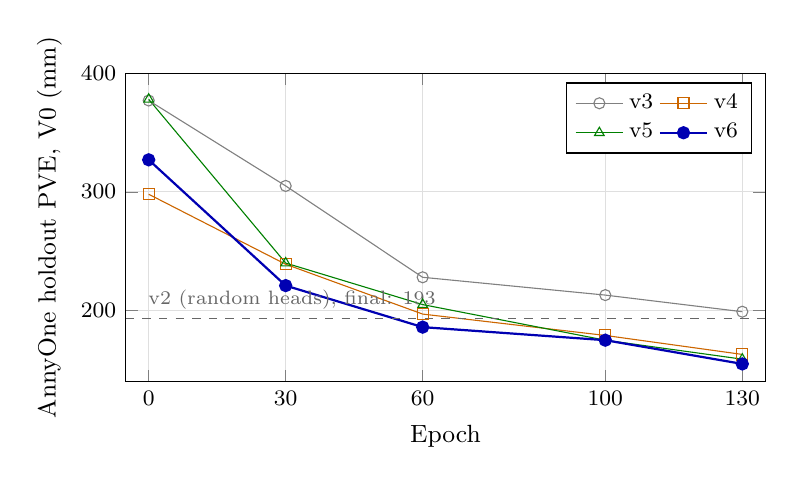
\begin{tikzpicture}
\begin{axis}[
  width=0.8\linewidth, height=5.5cm,
  xlabel={Epoch}, ylabel={AnnyOne holdout PVE, V0 (mm)},
  xmin=-5, xmax=135, ymin=140, ymax=400, xtick={0,30,60,100,130},
  grid=major, grid style={gray!25},
  tick label style={font=\footnotesize}, label style={font=\small},
  legend style={font=\footnotesize, at={(0.98,0.97)}, anchor=north east}, legend columns=2,
]
\addplot[color=gray, mark=o] coordinates {(0,377) (30,305) (60,228) (100,213) (130,199)};
\addlegendentry{v3}
\addplot[color=orange!80!black, mark=square] coordinates {(0,298) (30,239) (60,197) (100,179) (130,163)};
\addlegendentry{v4}
\addplot[color=green!50!black, mark=triangle] coordinates {(0,378) (30,240) (60,205) (100,175) (130,159)};
\addlegendentry{v5}
\addplot[color=blue!70!black, mark=*, thick] coordinates {(0,327) (30,221) (60,186) (100,175) (130,155)};
\addlegendentry{v6}
\draw[dashed, black!60] (axis cs:-5,193) -- (axis cs:135,193) node[pos=0.02, anchor=south west, font=\scriptsize] {v2 (random heads), final: 193};
\end{axis}
\end{tikzpicture}
\caption{Held-out PVE of the ViT-S head-transfer students at equal epochs (setting V0; history, before the depth and
bone fixes and the corrected 3DPW labels). Each student adds one change to the previous one: v4 an HMR-trained
student backbone, v5 a 5-epoch head freeze, v6 projector-fed heads.}
\label{fig:vits-curves}
\end{figure}


